\documentclass[10pt]{article}
%\usepackage{mathtools,hyperref,booktabs,fullpage, txfonts}
%\usepackage[utopia]{mathdesign}     

\usepackage[table]{xcolor}
\usepackage{amsmath}
\usepackage{amsfonts}
\usepackage{amssymb}
\usepackage{hyperref}
\usepackage{longtable}
\usepackage{fullpage}
\usepackage{graphicx}
\usepackage{caption}

 
\definecolor{lightgray}{gray}{0.93}

\pagestyle{empty}
\setlength\parindent{0pt}
\renewcommand{\thefootnote}{\fnsymbol{footnote}}
 
\makeatletter
\renewcommand\section{\@startsection{section}{1}{\z@}%
                                  {-3.5ex \@plus -1ex \@minus -.2ex}%
                                  {2.3ex \@plus.2ex}%
                                  {\normalfont\bfseries}}
\makeatother


\begin{document}

{\large
  \begin{center}
    {\bf BILL OF MATERIALS  \\ 
         11/9/18 \\
    }
  \end{center}
}
 
{\small {\bf Note}:
This document contains pricing and sizing information for the materials used in the construction of the Bonner tubes.}

\section*{Materials}

\href{https://www.onlinemetals.com/merchant.cfm?pid=12805&step=4&showunits=inches&id=946&top_cat=60}{Aluminum Tube}

\$34.56

.75", .652", 36" Length

\vspace{1cm}

\href{https://www.onlinemetals.com/merchant.cfm?pid=7685&step=4&showunits=inches&id=288&top_cat=60}{Solid Tubing for Holder/Plug}

\$8.18

.625" OD, 24" Length

\vspace{1cm}

\href{https://www.eplastics.com/HDPEBLK0125SR24X48}{HDPE}

\$16.02

24" x 48" x .125"

\vspace{1cm}

\href{https://www.grainger.com/product/MORSE-5-8-Dia-Hole-Saw-for-Masonry-40L157}{Hole Saw}

\$25.20

Diamond 5/8" Diameter Hole Saw 

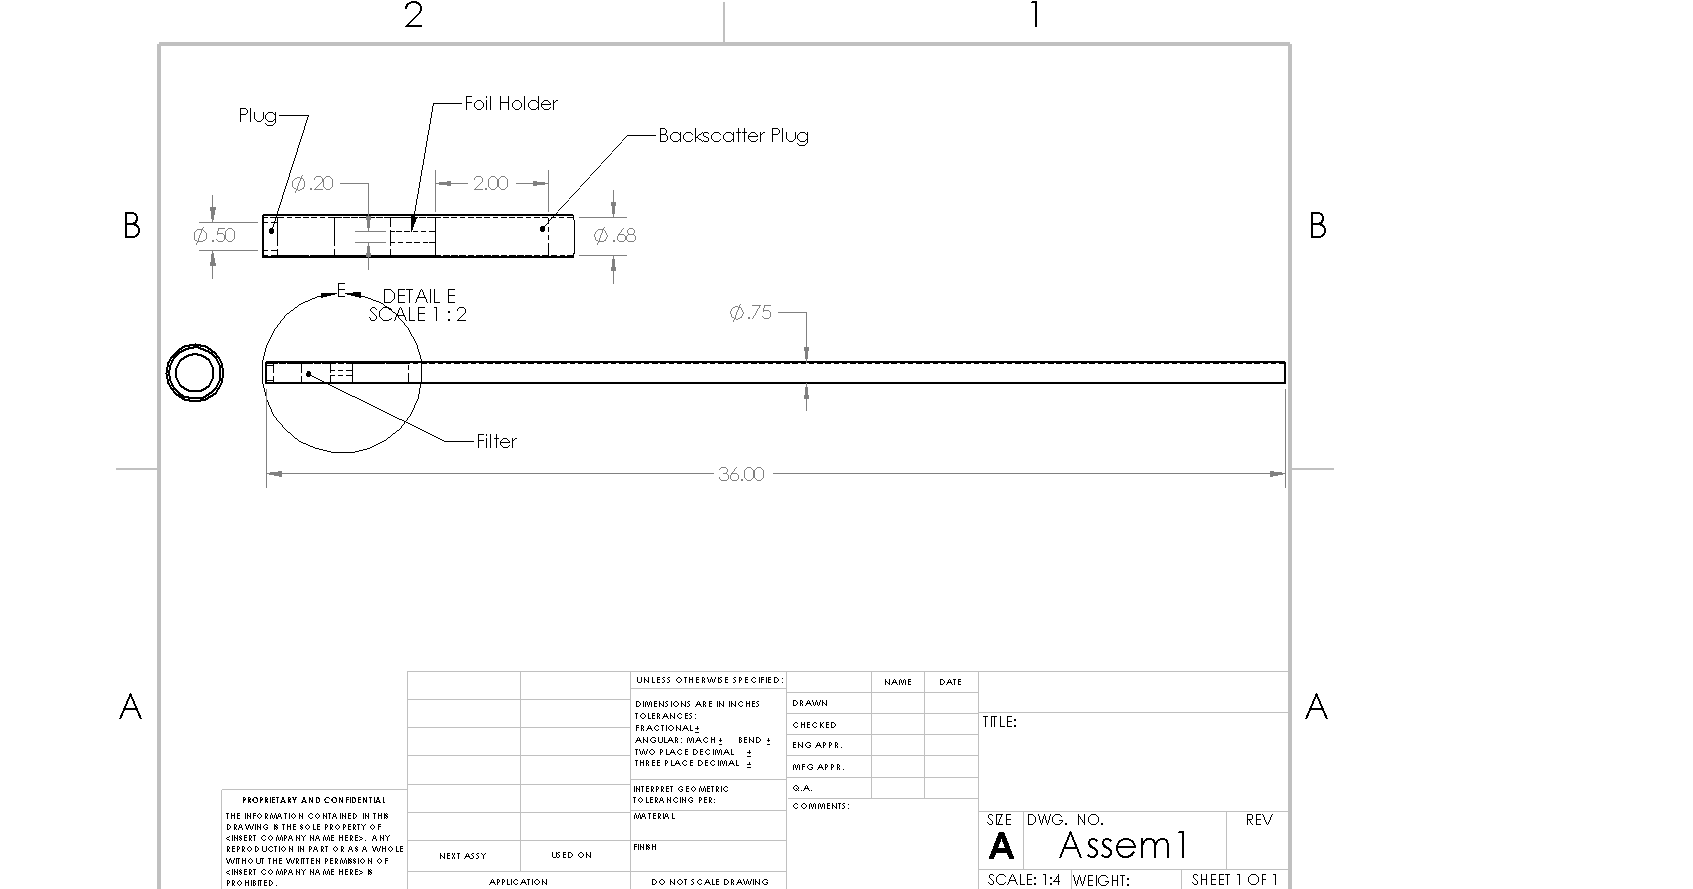
\includegraphics[width=20cm]{drawing.png}
\end{document}

    

